%%%%%%%%%%%%%%%%%%%%%%%%%%%%%%%%%%%%%%%%%
% Beamer Presentation
% LaTeX Template
% Version 1.0 (10/11/12)
%
% This template has been downloaded from:
% http://www.LaTeXTemplates.com
%
% License:
% CC BY-NC-SA 3.0 (http://creativecommons.org/licenses/by-nc-sa/3.0/)
%
%%%%%%%%%%%%%%%%%%%%%%%%%%%%%%%%%%%%%%%%%

%----------------------------------------------------------------------------------------
%	PACKAGES AND THEMES
%----------------------------------------------------------------------------------------

\documentclass{beamer}

\mode<presentation> {

% The Beamer class comes with a number of default slide themes
% which change the colors and layouts of slides. Below this is a list
% of all the themes, uncomment each in turn to see what they look like.

%\usetheme{default}
%\usetheme{AnnArbor}
%\usetheme{Antibes}
%\usetheme{Bergen}
%\usetheme{Berkeley}
%\usetheme{Berlin}
%\usetheme{Boadilla}
%\usetheme{CambridgeUS}
%\usetheme{Copenhagen}
%\usetheme{Darmstadt}
%\usetheme{Dresden}
%\usetheme{Frankfurt}
%\usetheme{Goettingen}
%\usetheme{Hannover}
%\usetheme{Ilmenau}
%\usetheme{JuanLesPins}
%\usetheme{Luebeck}
\usetheme{Madrid}
%\usetheme{Malmoe}
%\usetheme{Marburg}
%\usetheme{Montpellier}
%\usetheme{PaloAlto}
%\usetheme{Pittsburgh}
%\usetheme{Rochester}
%\usetheme{Singapore}
%\usetheme{Szeged}
%\usetheme{Warsaw}

% As well as themes, the Beamer class has a number of color themes
% for any slide theme. Uncomment each of these in turn to see how it
% changes the colors of your current slide theme.

%\usecolortheme{albatross}
%\usecolortheme{beaver}
%\usecolortheme{beetle}
%\usecolortheme{crane}
%\usecolortheme{dolphin}
%\usecolortheme{dove}
%\usecolortheme{fly}
%\usecolortheme{lily}
%\usecolortheme{orchid}
%\usecolortheme{rose}
%\usecolortheme{seagull}
%\usecolortheme{seahorse}
%\usecolortheme{whale}
%\usecolortheme{wolverine}

%\setbeamertemplate{footline} % To remove the footer line in all slides uncomment this line
%\setbeamertemplate{footline}[page number] % To replace the footer line in all slides with a simple slide count uncomment this line

%\setbeamertemplate{navigation symbols}{} % To remove the navigation symbols from the bottom of all slides uncomment this line
}

\usepackage{graphicx} % Allows including images
\usepackage{booktabs} % Allows the use of \toprule, \midrule and \bottomrule in tables

%----------------------------------------------------------------------------------------
%	TITLE PAGE
%----------------------------------------------------------------------------------------

\title[Cooperative Explorer]{COEX-1} % The short title appears at the bottom of every slide, the full title is only on the title page
\subtitle{Cooperative Explorer}
\author[Aurélien Werenne]{Aurélien Werenne \\ {\small Advisor: Prof. B. Boigelot}} 
\institute[ULiège] 
{
University of Liège \\ 
\medskip
}
\date{\today} 

\begin{document}

\begin{frame}
\titlepage 
\end{frame}

\begin{frame}
\frametitle{Overview} 
\tableofcontents 
\end{frame}

%----------------------------------------------------------------------------------------
%	PRESENTATION SLIDES
%----------------------------------------------------------------------------------------

%------------------------------------------------
\section{General} 
%------------------------------------------------

\begin{frame}
\frametitle{General}
\framesubtitle{Objective}
The goal of the robot is to map an unknown environment in a centralized multi-agent setting.\\~\\
The main features of the robots are:
\begin{itemize}
\item Following a black line
\item Computing the travelled distance
\item Detecting, classifying and handling intersections
\item Avoiding obstacles
\item Communicating with a central unit 
\end{itemize}
\end{frame}

%------------------------------------------------

\begin{frame}
\frametitle{General}
\framesubtitle{Material}
\begin{itemize}
\item Arduino Nano 
\item Reflectance sensor array 
\item Sharp sensor 
\item Magnetic encoders 
\item Pololu micro metal gearmotor 
\item L298 dual H-bridge 
\item NiMH Battery 7.2V 
\item HC-06 Bluetooth module 
\item ...
\end{itemize}
\end{frame}

%------------------------------------------------

\begin{frame}
\frametitle{General}
\framesubtitle{Structure (1/3)}
\begin{figure}[hbtp]
\centering
\includegraphics[scale=0.05]{figures/img_front.JPG}
\caption{Front view of COEX-1}
\end{figure}
\end{frame}

%------------------------------------------------

\begin{frame}
\frametitle{General}
\framesubtitle{Structure (2/3)}
\begin{figure}[hbtp]
\centering
\includegraphics[scale=0.05]{figures/img_side.JPG}
\caption{Side view of COEX-1}
\end{figure}
\end{frame}

%------------------------------------------------

\begin{frame}
\frametitle{General}
\framesubtitle{Structure (3/3)}
\begin{figure}[hbtp]
\centering
\includegraphics[scale=0.05]{figures/img_bottom.JPG}
\caption{Bottom view of COEX-1}
\end{figure}
\end{frame}

%------------------------------------------------

\begin{frame}
\frametitle{General}
\framesubtitle{Variables}
\begin{itemize}
\item List of variables used in equations with small explanations
\end{itemize}
\end{frame}

%------------------------------------------------
\section{Components} 
%------------------------------------------------

\begin{frame}
\frametitle{Components}
\framesubtitle{Sharp sensor}
Explain flow test. Conclusion.
\begin{figure}[hbtp]
\centering
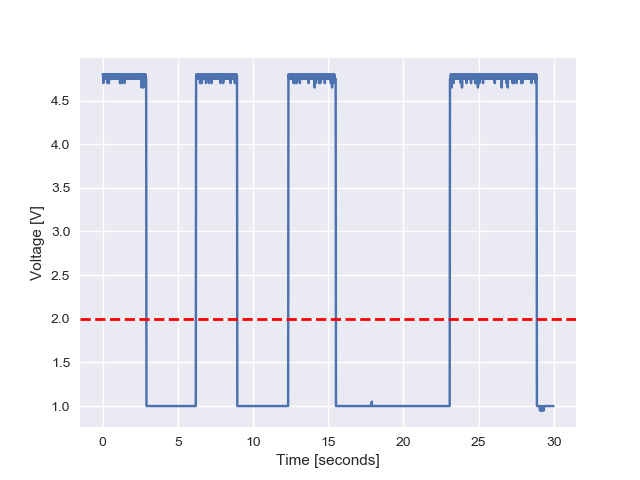
\includegraphics[scale=0.4]{figures/sharp-flow.png}
\caption{Obstacle movement (alternating between in and out of reach of sensor)}
\end{figure}
\end{frame}


%------------------------------------------------

\begin{frame}
\frametitle{Components}
\framesubtitle{Reflectance sensor array (line sensor)}
Explain flow test. Explain err line.Conclusion.
\begin{figure}[hbtp]
\centering
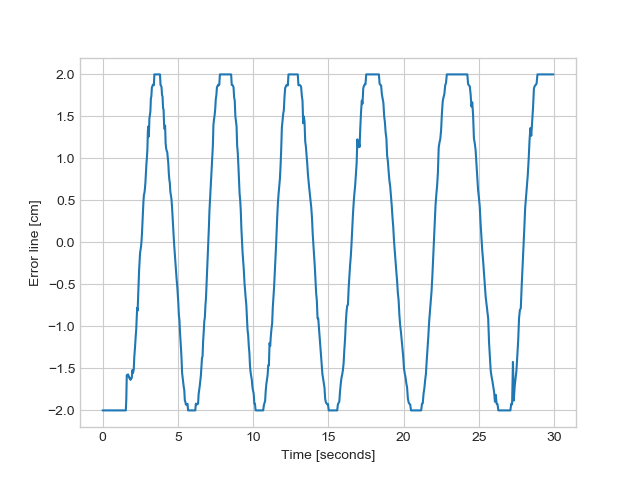
\includegraphics[scale=0.4]{figures/qtr-flow.png}
\caption{Obstacle movement (alternating between in and out of reach of sensor)}
\end{figure}
\end{frame}

%------------------------------------------------

\begin{frame}
\frametitle{Components}
\framesubtitle{Shield}
The line sensors are fixed vertically well above the given recommendations, such that the robot has place to climb hills. This decision made the line sensor 
particularly sensitive to ambient light interferences. Thus a shield had to be constructed. Explain after wheel. \\~\\
\end{frame}

%------------------------------------------------

\begin{frame}
\frametitle{Components}
\framesubtitle{Bluetooth module (1/2)}
Explain sender-receiver distortion.\\~\\
Plots.\\~\\
Conclusion.
\end{frame}

%------------------------------------------------

\begin{frame}
\frametitle{Components}
\framesubtitle{Bluetooth module (2/2)}
Logic level Arduino is 0 5 and HC 05 module is 0 3.3 V..
\begin{columns}[c]

\column{.35\textwidth}
\begin{align*} 
V_{arduino} &=  \frac{R_2}{R_1+R_2}V_{blt} \\[0.4cm]
 &=  \frac{2.2}{3.2}V_{blt}
\end{align*}

\column{.65\textwidth}
\begin{figure}[hbtp]
\centering
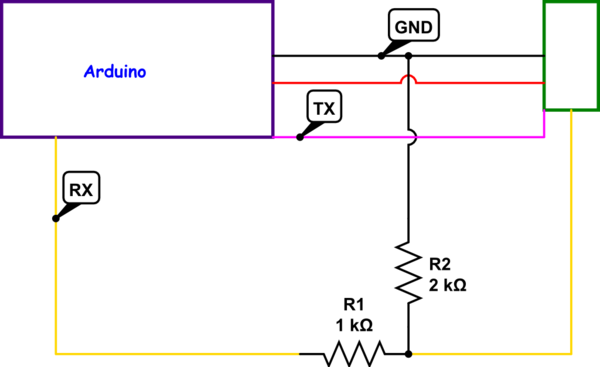
\includegraphics[scale=0.5]{figures/voltage-divider.png}
\caption{Voltage divider}
\end{figure}

\end{columns}
\end{frame}

%------------------------------------------------

\begin{frame}
\frametitle{Components}
\framesubtitle{Quadrature encoders (1/2)}
$$ 
w_L = 2\pi f_L
\qquad\text{with}\qquad	
f_L = \frac{n_L}{N' \, G_b \, \Delta{t} }
$$
$$ 
v = \frac{v_L + v_R}{2} = \frac{R(w_L + w_R)}{2}
$$
\end{frame}

%------------------------------------------------

\begin{frame}
\frametitle{Components}
\framesubtitle{Quadrature encoders (2/2)}
Remark why divide by 2 for counting. because only 2 pin interrupts.
\end{frame}

%------------------------------------------------

\begin{frame}
\frametitle{Components}
\framesubtitle{Motors}
Conclusion. Need for regulation. Two more curves on same plot but with full/empty battery.
\begin{figure}[hbtp]
\centering
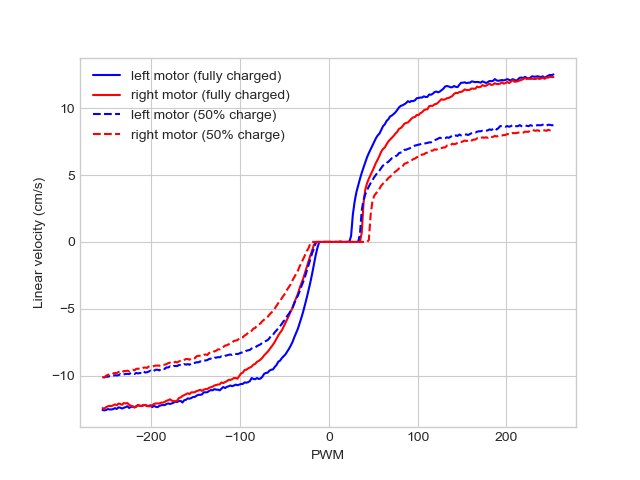
\includegraphics[scale=0.4]{figures/motors_merged.png}
\caption{Relationship between PWM (input) and measured speed (output)}
\end{figure}

\end{frame}


%------------------------------------------------
\section{Control} 
%------------------------------------------------

\begin{frame}
\frametitle{Control}
\framesubtitle{General framework}
Use of classical PID controller.
$$ 
o_n \leftarrow K_p e_n + K_d\frac{e_n - e_{n-1}}{\Delta t_{n-1:n}} + K_e\sum_{i=0}^{n}{e_i \Delta t_{n-1:n}}
$$
with the following two precautions called respectively anti-windup and anti-derivative kick:
$$
o_n = \left\{
    \begin{array}{ll}
        max & \mbox{if } o_n > max \\
        min & \mbox{if } o_n < min \\
        o_n & \mbox{otherwise.}
    \end{array}
\right.
\qquad\text{and}\qquad	
K_d = \left\{
    \begin{array}{ll}
        0 & \mbox{if } n < T \\
       K_d & \mbox{otherwise.}
    \end{array}
\right.
$$
\end{frame}

%------------------------------------------------

\begin{frame}
\frametitle{Control}
\framesubtitle{Speed \& direction}
$$ 
\left\{
    \begin{array}{ll}
		\alpha = o(e_{direction}) \\[0.3cm]
		\beta = o(e_{speed}) \\[0.3cm]
		\gamma = o(e_{align})
	\end{array}
\right.
\Rightarrow
\left\{
    \begin{array}{ll}
		{pwm}_L =  (\beta -\gamma) + \alpha \\
		{pwm}_R = (\beta - \gamma) - \alpha
	\end{array}
\right.
$$
\end{frame}

%------------------------------------------------

\begin{frame}
\frametitle{Control}
\framesubtitle{Line-following control}
Recall plot of sensor. 
$$ 
e_{direction} =err_{line} \in [-2500;2500]
$$
Explain perturbation plot.\\~\\
Perturbation plot.\\~\\
Conclusion. break out angle. Agressive enough such that not seen as intersection.
\end{frame}

%------------------------------------------------

\begin{frame}
\frametitle{Control}
\framesubtitle{Speed control (1/4)}
Reason. Target and progress speed.
$$
v_{n+1} \leftarrow v_n + A \, \Delta t_{n:n+1}
$$
\begin{align*}
&\Leftrightarrow \int_{0}^{T}a(t) =  \int_{0}^{T}a'(t) \\
&\Leftrightarrow A\,T = \underbrace{d\,B}_{triangles} + \underbrace{(T - 2d)B}_{rectangle}
\end{align*}
We introduce the parameter $\psi = \frac{d}{T}$ such that
$$
\boxed{B = \frac{A}{1-\psi}} 
$$
\end{frame}

%------------------------------------------------

\begin{frame}
\frametitle{Control}
\framesubtitle{Speed control(2/4)}
$$
v_{n+1} \leftarrow v_n + \int_{n}^{n+1}a'(t) = v_n + \int_{0}^{n+1}a'(t) - \int_{0}^{n}a'(t)
$$
Diagrams.
\end{frame}

%------------------------------------------------

\begin{frame}
\frametitle{Control}
\framesubtitle{Speed control (3/4)}
Reason.\\~\\
Target and progress speed.\\~\\
Equations.\\~\\
Diagrams.
\end{frame}

%------------------------------------------------

\begin{frame}
\frametitle{Control}
\framesubtitle{Speed control (4/4)}
Explain plot.\\~\\
PID plot.\\~\\
Conclusion. Room for fine-tuning.
\end{frame}

%------------------------------------------------

\begin{frame}
\frametitle{Control}
\framesubtitle{Forward}
Explain forward. Explain improvement would be to consider theta instead.\\~\\
$$
e_{direction} = v_R - v_L
$$
We verify that if
$$
v_{R;n} > v_{L;n} \Rightarrow e_n > 0  \Rightarrow \alpha_n > 0  \Rightarrow v_{R;n+1}\uparrow \, , v_{L;n+1}\downarrow
$$
\end{frame}

%------------------------------------------------

\begin{frame}
\frametitle{Control}
\framesubtitle{Turning (1/2)}
From Fig. we can easily deduce the model below by integrating the angular velocity .
$$
\theta(t) = \frac{2vt}{b} + \theta_0
\qquad\text{because}\qquad	
v_R = -v_L
$$
\begin{figure}[hbtp]
\centering
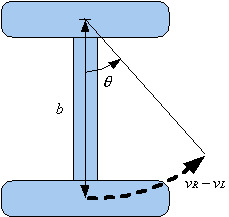
\includegraphics[scale=0.5]{figures/differential-system.jpg}
\end{figure}
\end{frame}

%------------------------------------------------

\begin{frame}
\frametitle{Control}
\framesubtitle{Turning (2/2)}
$$
\theta_{n+1} \leftarrow \frac{2\, v_n\, \Delta_{n:n+1}}{b}
$$
PID. 
\end{frame}


%------------------------------------------------
\section{Exploration \& Mapping} 
%------------------------------------------------

%------------------------------------------------

\begin{frame}
\frametitle{Exploration \& Mapping}
\framesubtitle{General}
To explore an unknown environment structured as a maze it needs to be able to:
\begin{itemize}
\item Compute the distance travelled since the last intersection
\item Detect an intersection
\item Turn to the desired intersection
\end{itemize}
\end{frame}

%------------------------------------------------

\begin{frame}
\frametitle{Exploration \& Mapping}
\framesubtitle{Distance (1/5)}
First method: Simple equation - explain without mathematics.\\~\\
Second method: Upperbound of error can be reduced due to relation with distance.\\~\\
plot relationship
\end{frame}

%------------------------------------------------

\begin{frame}
\frametitle{Exploration \& Mapping}
\framesubtitle{Distance (2/5)}
Plot comparison with error bars of two methods on test set.\\~\\
Conclusion.
\end{frame}

%------------------------------------------------

\begin{frame}
\frametitle{Exploration \& Mapping}
\framesubtitle{Distance (3/5)}
Explain we could try to quantify uncertainty and above certain threshold not accept it.\\~\\
$$
	MSE = \sum_{i=0}^N err_{line}^2
$$
obtained iteratively by rolling mean method.
One plot 
\end{frame}

%------------------------------------------------

\begin{frame}
\frametitle{Exploration \& Mapping}
\framesubtitle{Distance (4/5)}
Explain simpler choice is to discretize from second method discretization.\\~\\
Remard 7.5-12.5 ....\\~\\
Plot discretization on test set.
\end{frame}

%------------------------------------------------

\begin{frame}
\frametitle{Exploration \& Mapping}
\framesubtitle{Distance (5/5)}
Example of resulting big map. Explain annotation\\~\\
Map.
\end{frame}

%------------------------------------------------

\begin{frame}
\frametitle{Exploration \& Mapping}
\framesubtitle{Intersection detection}
Explain problem of naive approach.\\~\\
$$
y = \underset{x \in  \{0,1\}}{\operatorname{argmax}} \operatorname{mode}(x)
$$
Boolean value for intersection based on decision rule as follows
$$
(y_C = 0) \lor (y_L = 1) \lor (y_R = 1) \lor (y_F = 0) 
$$
\end{frame}

%------------------------------------------------

\begin{frame}
\frametitle{Exploration \& Mapping}
\framesubtitle{Intersection classification}
Explain classification.\\~\\
Figures of 8 types.\\~\\
\end{frame}

%------------------------------------------------

\begin{frame}
\frametitle{Exploration \& Mapping}
\framesubtitle{Turning \& alignment (1/2)}
Problem with naive approach.\\~\\
Solution + plot + equation.
\end{frame}

%------------------------------------------------

\begin{frame}
\frametitle{Exploration \& Mapping}
\framesubtitle{Turning \& alignment (2/2)}
Explain plot.\\~\\
Plot to verify results.\\~\\
Conclusion.
\end{frame}

%------------------------------------------------
\section{Code} 
%------------------------------------------------

\begin{frame}
\frametitle{Code}
\framesubtitle{General architecture}
Advantage.\\~\\
Diagram.\\~\\
Link to code.\\~\\
\end{frame}

%------------------------------------------------

\begin{frame}
\frametitle{Code}
\framesubtitle{Pseudo-code exploration}
Pseudocode.\\~\\
\end{frame}


%------------------------------------------------

\begin{frame}
\begin{figure}[hbtp]
\centering
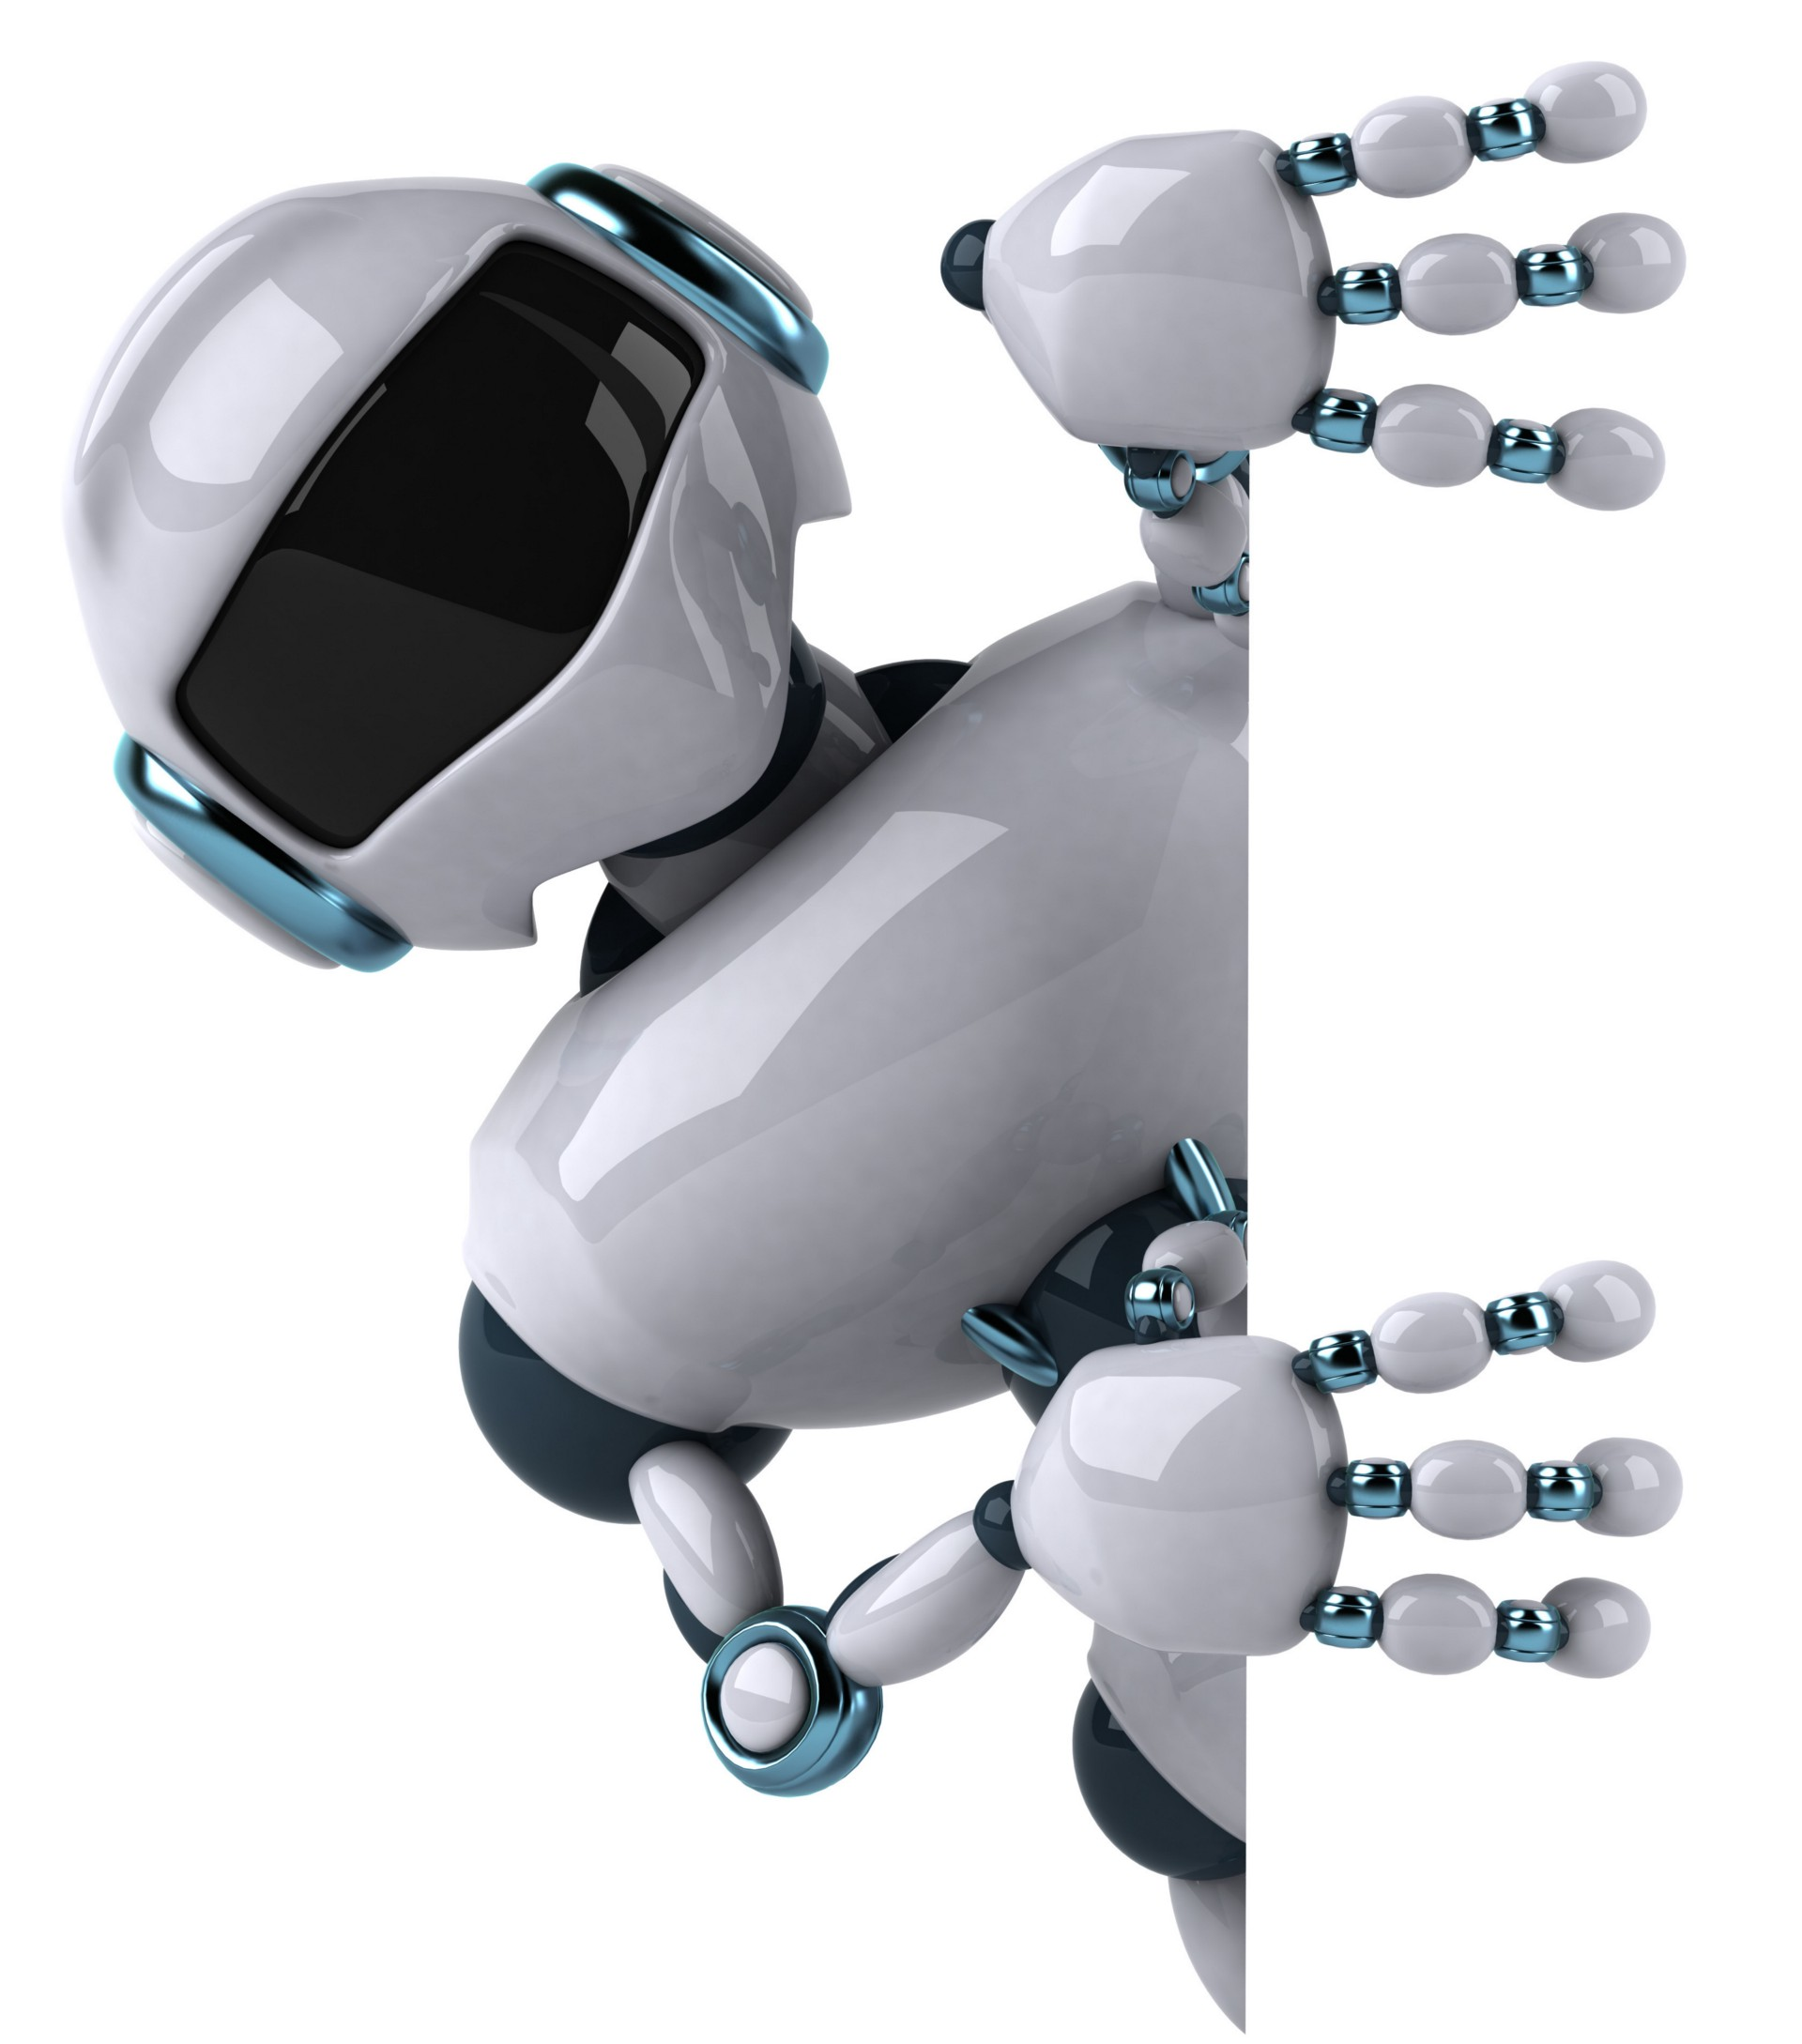
\includegraphics[scale=0.1]{figures/bye-bye.jpeg}
\end{figure}
\end{frame}

%----------------------------------------------------------------------------------------

\end{document}